
% On définit le type de document, de papier et la grosseur des caractères.
\documentclass[letterpaper,11pt]{article}

% Trois lignes liées à l'ordinateur avec lequel on produit le document.
\usepackage[utf8]{inputenc}
\usepackage{titling}
\usepackage{amsthm}

% Highlight text
\usepackage{soul} % for the command \hl

% Bibliographie
\usepackage[
backend=biber,
style=alphabetic,
sorting=ynt
]{biblatex}
\addbibresource{Bib1.bib}

\usepackage{dsfont}
\usepackage{layout}
\usepackage{cancel}
\usepackage[french]{babel}
\usepackage[T1]{fontenc}
\usepackage[utf8]{inputenc}
\usepackage[document]{ragged2e}
\usepackage[top=2cm,bottom=2cm,left=2.5cm,right=2.5cm,includehead=true,headheight=1cm]{geometry}%Pour ajustement des marges.
\usepackage{amsbsy}%Accès à des symboles mathématiques
\usepackage{amsfonts}%Accès à des symboles mathématiques
\usepackage{amssymb}%Accès à des symboles mathématiques
\usepackage{bm}%Pour mettre en gras n'importe quel symbole.
\usepackage{enumerate}%Pour les listes d'énumération.
\usepackage{parskip}%Pour pouvoir modifier l'espace entre les paragraphes.
\usepackage{setspace}%Pour pouvoir modifier l'espace entre les lignes.
\usepackage{upgreek}%Pour accéder aux lettres grecques en romain.
\usepackage[b]{esvect}%Permet de créer des vecteurs.
\usepackage{wasysym}
\usepackage{afterpage}
\usepackage{ stmaryrd }
\usepackage{minted}
\usepackage{mathtools}
\usepackage{placeins}
\usepackage{hyperref}
\usepackage{csvsimple}
\usepackage{adjustbox}
\usepackage{booktabs}
\usepackage{rotating}
\usepackage{colortbl}
\usepackage{xcolor}
%Symboles fréquents
\newcommand{\N}{\mathbb{N}}
\newcommand{\R}{\mathbb{R}}
\newcommand{\C}{\mathbb{C}}
\newcommand{\I}{\mathbb{I}}
\newcommand{\Z}{\mathbb{Z}}
\newcommand{\Q}{\mathbb{Q}}
\newcommand{\E}{\mathbb{E}}
\newcommand{\?}{\stackrel{?}{=}}
\let\epsilon\varepsilon
\newcommand{\der}{\text{d}}

\newcommand{\macroA}[1]{y_{#1}^{(1*)}}
\newcommand{\macroB}[1]{y_{#1}^{(1)}}
\newcommand{\macroC}[1]{r_{#1,fx}}

%Mettre en gras ET italique le paramètre de la fonction
\newcommand{\gras}[1]{\textbf{\textit{#1}}} 

\newcommand\blankpage{%
    \null
    \thispagestyle{empty}%
    \addtocounter{page}{-1}%
    \newpage}%page vierge


\newcommand{\probVar}[1]{\text{Var}\left(#1\right)} %Variance
\newcommand{\probCov}[1]{\text{Cov}\left(#1\right)} %Variance
\newcommand{\probP}[1]{\mathds{P}\left{#1\right}} %P de probabilités
\newcommand{\probE}[1]{\mathbb{E}\left[#1\right]} %E de espérance

\usepackage{hyperref}%'Linker' des équations et sources

%Les quatre lignes qui suivent définissent l'espace entre les paragraphes, l'indentation, l'espace entre les lignes et la distance entre une boite et ce qu'elle contient.
\parskip=10pt 
\parindent=0pt
\onehalfspacing
\fboxsep=9pt

%Parenthèses
\newcommand{\bgl}{\bigl(}
\newcommand{\Bgl}{\Bigl(}
\newcommand{\bggl}{\biggl(}
\newcommand{\Bggl}{\Biggl(}
\newcommand{\bgr}{\bigr)}
\newcommand{\Bgr}{\Bigr)}
\newcommand{\bggr}{\biggr)}
\newcommand{\Bggr}{\Biggr)}

\renewcommand\thesection{\arabic{section}}
\renewcommand\thesubsection{\thesection.\arabic{subsection}}

\begin{document}

\begin{titlepage}
    \centering
    
\includegraphics[width=0.3\textwidth]{udem.png}\par\vspace{1cm} % Replace with your logo file
    {\scshape\LARGE Université de Montréal \par}
    \vspace{1cm}
    {\scshape\Large Département de Sciences Économiques\par}
    \vspace{1.5cm}
    {\huge\bfseries Rapport Devoir 3\par}
    \vspace{1.5cm}
    {\Large\itshape Nguyen-Xuan-Bach Bui\par}
    \vfill
    {\Large ECN 6258 - Sujets spéciaux en monnaie, banques et marchés\par}
\end{titlepage}

All codes are available at \url{https://github.com/BNXBach/Work_stuffs_A2025/tree/main/TP_ECN}

\section*{Question 3: Comment sont créées les obligations STRIPs? Quelle organisation gère ce
processus au Canada?}

Extrait directement de \cite{web}, on a les étapes de création des obligations STRIPS:

Les obligations STRIPs sont créées en séparant les paiements d’intérêts (coupons) du remboursement du capital d’une obligation à coupon classique. Ce processus, appelé "découpage" ou "stripping" en anglais, consiste à diviser l’obligation en ses composantes : les coupons individuels et le solde de l’obligation (le montant du capital). Chaque composante peut ensuite être vendue séparément comme une obligation à coupon zéro.

Par exemple, prenons une obligation du gouvernement du Canada à 10 ans d’une valeur nominale de 1 000\$ et d’un taux de coupon annuel de 5 \%. Cette obligation peut être découpée en 10 paiements de coupons distincts de 50\$ chacun et un paiement unique de capital de 1 000\$. Chacun de ces composants peut être vendu individuellement sous forme d'obligation STRIP.


Au Canada, l'organisation principal qui gère les obligations STRIPs est le Canadian Depository for Securities (CDS) 

Lien des rapports des obligations STRIPs:\url{https://www.cds.ca/participants/settlement-and-clearing/strip-bond-reports?lang=en}


\newpage
\section*{Question 6: Comment calcule-t-on la durée et la convexité de cette obligation?}
Comme les obligations STRIPs sont un type de l'obligation zéro coupon, on peut utiliser directement le résultat dans \cite{book}:
\begin{itemize}
    \item Durée: $D=T-t$
    \item Convexité: $C= (T-t)^2$
\end{itemize}

Dans notre fichier "StripCouponYield.xlsx", la valeur $T-t$ est donnée dans la feuille "maturity" alors on peut l'utiliser directement.

\newpage
\section*{Question 7+8: Immunisation dynamique 1 et 2}
\subsection*{Préliminaire}
Premièrement, on veut montrer d'abord que la stratégie d'immunisation 1 dans l'énoncé n'est pas celle dans \cite{book} et en fait n'est pas un portefeuille qui immunise la durée:

Soit $D$ la durée de l'obligation cible, $C$ sa convexité et $P$ son prix. De même, on peut définir $D_{short}$, $D_{long}$, $C_{short}$, $C_{long}$, $P_{short}$, $P_{long}$ pour les 2 obligations longue et courte. Soit $q$ la quantité nécessaire de l'obligation longue pour immuniser la durée.

Le portefeuille mentionné dans \cite{book} dans notre cas sera:
\begin{equation*}
    \begin{aligned}
        V &=P+P_{short}+qP_{long} \\
      \Rightarrow{} \ D_V&=DP+D_{short}P_{short}+qD_{long} P_{long} =0 \\
      \Rightarrow{} \ q&= \dfrac{-DP-D_{short}P_{short}}{D_{long} P_{long}} \\
    \end{aligned}
\end{equation*}

En fait, pour immuniser la durée de l'obligation cible, il faut qu'on l'inclut dans le portefeuille. Alors, le portefeuille dans l'énoncé du TP ne va pas immuniser la durée de l'obligation cible. 
De plus, considérons ce portefeuille qu'on appelle $V^*$:

\begin{equation*}
    \begin{aligned}
        V^* &=P_{short}+q^*P_{long} \\
      \Rightarrow{} \ D_V &=D_{short}P_{short}+qD_{long} P_{long} =D \\
      \Rightarrow{} \ q^* &= \dfrac{-D-D_{short}P_{short}}{D_{long} P_{long}} \\
    \end{aligned}
\end{equation*}

On note que $q$ et $q^*$ sont différents alors même si on construit le portefeuille de l'énoncé de TP avec $q^*$ et puis faire $V^{**} = V^*-P$, on n'aura pas un portefeuille immunisant la durée de l'obligation cible.

En réalité, ce que le portefeuille de l'énoncé fait, c'est adapter sa durée à celle de l'obligation cible. C'est utile si on n'a pas l'accès à l'obligation cible et on veut créer un portefeuille qui a sa durée mais si le but est de créer un portefeuille immunisant la durée, ce portefeuille n'est pas le choix.

De plus, dans la stratégie immunisation dynamique 2, c'est écrit dans l'énoncé d'utiliser les poids donnés dans \cite{book} qui donne ce portefeuille $V = P+k_1P_{short}+k_2P_{long}$. Alors, afin de comparer les deux portefeuilles de manière logique, pour la stratégie immunisation dynamique 1, on suivra \cite{book} et pas l'énoncé du TP.

\newpage
Deuxièment, on manque quelques informations nécessaires pour faire les calculs, notamment:
\begin{itemize}
    \item La compostion des taux d'intérêts. La composition des taux changera le prix de l'obligation ce qui est nécessaire pour calculer les poids. Dans notre fichier code, on a inclu l'option de choisir quel type de composition on veut utiliser. Pour ce rapport, on va montrer seulement le cas où la composition est annuelle et donc le prix est $P=\dfrac{1}{(1+r)^{T-t}}$. La raison est parce qu'on a déjà testé les 2 cas et la conclusion est identique.
    \item La duplication de l'obligation longue
    \begin{figure}[H]
    \centering
    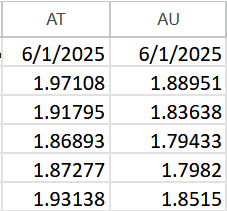
\includegraphics[width=0.4\columnwidth]{duplication.png}
    \caption{Il y a 2 obligations longues avec la maturité qu'on veut}
\end{figure}
\FloatBarrier
    On assume qu'il y a 2 obligations qui ont la même maturité alors on peut choisir une parmi ces deux. Dans notre fichier code, il y a aussi un choix entre ces 2 obligations. Pour ce rapport, on montre seulement le cas où on choisit l'obligation long 1 (colonne AT). La raison est la même, on a déjà testé avec l'obligation long 2 et la conclusion est identique.
\end{itemize}

\newpage
\subsection*{Résultat}
On a construit les 2 portefeuiles $V_1=P+P_{short}+qP_{long}$ qui immunise la durée et $V_2=P+k_1P_{short}+k_2P_{long}$ qui immunise la durée et la convexité. Pour montrer les résultats des deux portefeuilles, on donne un tableau avec 10 colonnes:
\begin{itemize}
    \item Date: La date actuelle (temps $t$)
    \item $q$: La quantité de l'obligation longue pour immuniser la durée de $V_1$
    \item \bm{$\textbf{PV}_1^{current}$}: La valeur du portefeuille $V_1$ au temps $t$
    \item \bm{$\textbf{PV}_1^{next}$}: La valeur du portefeuille $V_1$ au temps $t+1$
    \item \bm{$\textbf{Difference PV}_1$}: La différence entre les 2 valeurs du portefeuille $V_1$ au temps $t+1$ et $t$ 
    \item $k_1$: La quantité de l'obligation courte pour immuniser la durée et la convexité de $V_2$
    \item $k_2$: La quantité de l'obligation longue pour immuniser la durée et la convexité de $V_2$
    \item \bm{$\textbf{PV}_2^{current}$}: La valeur du portefeuille $V_2$ au temps $t$
    \item \bm{$\textbf{PV}_2^{next}$}: La valeur du portefeuille $V_2$ au temps $t+1$
    \item \bm{$\textbf{Difference PV}_2$}: La différence entre les 2 valeurs du portefeuille $V_2$ au temps $t+1$ et $t$ 
\end{itemize}

Voici le tableau de résultat:

\begin{table}[htbp]
\centering
\begin{adjustbox}{width=1.2\textwidth,center=\textwidth}
\begin{tabular}{ l  *9c }
\toprule
\textbf{Date} & \textbf{q} & \bm{$\textbf{PV}_1^{current}$} & \bm{$\textbf{PV}_1^{next}$} & \bm{$\textbf{Difference PV}_1$} & \bm{$k_1$} & \bm{$k_2$} & \bm{$\textbf{PV}_2^{current}$} & \bm{$\textbf{PV}_2^{next}$} & \bm{$\textbf{Difference PV}_2$} \\
\midrule
\rowcolor{black!10}08-Jan-2015 & -0.890313 & 1.166884 & 1.163833 & -0.003051 & -1.31747 & -0.25314 & -0.572136 & -0.571207 & 0.000929 \\
15-Jan-2015 & -0.873877 & 1.177617 & 1.187815 & 0.010198 & -1.334947 & -0.249475 & -0.585249 & -0.586172 & -0.000924 \\
\rowcolor{black!10}22-Jan-2015 & -0.872956 & 1.188593 & 1.186555 & -0.002038 & -1.34531 & -0.249801 & -0.596661 & -0.595311 & 0.00135 \\
29-Jan-2015 & -0.861458 & 1.196429 & 1.196804 & 0.000375 & -1.360249 & -0.247338 & -0.607954 & -0.608208 & -0.000255 \\
\rowcolor{black!10}05-Feb-2015 & -0.858007 & 1.199774 & 1.200629 & 0.000855 & -1.36753 & -0.246744 & -0.614896 & -0.615752 & -0.000857 \\
12-Feb-2015 & -0.856809 & 1.201657 & 1.203646 & 0.001989 & -1.372361 & -0.24666 & -0.620457 & -0.621501 & -0.001043 \\
\rowcolor{black!10}19-Feb-2015 & -0.857956 & 1.202667 & 1.196821 & -0.005846 & -1.375643 & -0.247168 & -0.625179 & -0.622155 & 0.003024 \\
26-Feb-2015 & -0.848644 & 1.204841 & 1.206848 & 0.002007 & -1.38882 & -0.245182 & -0.633452 & -0.633894 & -0.000443 \\
\rowcolor{black!10}05-Mar-2015 & -0.854962 & 1.201499 & 1.203142 & 0.001643 & -1.388277 & -0.246978 & -0.63488 & -0.633666 & 0.001214 \\
12-Mar-2015 & -0.851577 & 1.206018 & 1.202203 & -0.003814 & -1.398923 & -0.246559 & -0.643801 & -0.643191 & 0.00061 \\
\rowcolor{black!10}19-Mar-2015 & -0.838837 & 1.213224 & 1.21284 & -0.000384 & -1.41406 & -0.243643 & -0.655615 & -0.656606 & -0.000991 \\
26-Mar-2015 & -0.841105 & 1.2109 & 1.210222 & -0.000678 & -1.41505 & -0.244352 & -0.658188 & -0.657336 & 0.000852 \\
\rowcolor{black!10}02-Apr-2015 & -0.832226 & 1.217916 & 1.219457 & 0.001541 & -1.429419 & -0.242489 & -0.66991 & -0.670551 & -0.000641 \\
09-Apr-2015 & -0.832831 & 1.218936 & 1.2163 & -0.002636 & -1.434138 & -0.242898 & -0.675562 & -0.675111 & 0.00045 \\
\rowcolor{black!10}16-Apr-2015 & -0.829033 & 1.219572 & 1.22081 & 0.001238 & -1.441693 & -0.24216 & -0.681923 & -0.682769 & -0.000845 \\
23-Apr-2015 & -0.832187 & 1.218124 & 1.222063 & 0.003939 & -1.443545 & -0.243172 & -0.685454 & -0.685795 & -0.000341 \\
\rowcolor{black!10}30-Apr-2015 & -0.836253 & 1.218637 & 1.222894 & 0.004258 & -1.447399 & -0.244548 & -0.690746 & -0.692293 & -0.001547 \\
07-May-2015 & -0.841309 & 1.218688 & 1.222365 & 0.003677 & -1.448974 & -0.246104 & -0.695137 & -0.695069 & 6.8e-05 \\
\rowcolor{black!10}14-May-2015 & -0.842909 & 1.221041 & 1.220185 & -0.000857 & -1.45591 & -0.246912 & -0.702562 & -0.702689 & -0.000127 \\
21-May-2015 & -0.838484 & 1.223854 & 1.223892 & 3.8e-05 & -1.465131 & -0.246062 & -0.711061 & -0.709261 & 0.0018 \\
\rowcolor{black!10}28-May-2015 & -0.831486 & 1.229752 & 1.234553 & 0.0048 & -1.480652 & -0.244743 & -0.723452 & -0.724826 & -0.001374 \\
04-Jun-2015 & -0.834417 & 1.232118 & 1.232607 & 0.000489 & -1.485563 & -0.245837 & -0.730578 & -0.730853 & -0.000275 \\
\rowcolor{black!10}11-Jun-2015 & -0.83546 & 1.231747 & 1.233327 & 0.00158 & -1.49051 & -0.246377 & -0.736171 & -0.734963 & 0.001208 \\
18-Jun-2015 & -0.831811 & 1.236346 & 1.236509 & 0.000163 & -1.503521 & -0.245903 & -0.7474 & -0.748806 & -0.001406 \\
\rowcolor{black!10}25-Jun-2015 & -0.829988 & 1.238014 & 1.240622 & 0.002609 & -1.509867 & -0.245655 & -0.75486 & -0.753359 & 0.0015 \\
02-Jul-2015 & -0.823286 & 1.246216 & 1.243522 & -0.002693 & -1.52791 & -0.244481 & -0.770219 & -0.768159 & 0.00206 \\
\rowcolor{black!10}09-Jul-2015 & -0.813501 & 1.251796 & 1.252462 & 0.000666 & -1.545889 & -0.242359 & -0.784153 & -0.784601 & -0.000447 \\
16-Jul-2015 & -0.809507 & 1.255848 & 1.254854 & -0.000994 & -1.557117 & -0.24165 & -0.795118 & -0.792413 & 0.002705 \\
\rowcolor{black!10}23-Jul-2015 & -0.803479 & 1.260001 & 1.255292 & -0.004708 & -1.573939 & -0.240555 & -0.808136 & -0.811325 & -0.003189 \\
30-Jul-2015 & -0.796997 & 1.260838 & 1.261308 & 0.00047 & -1.579661 & -0.23885 & -0.815532 & -0.813902 & 0.00163 \\
\rowcolor{black!10}06-Aug-2015 & -0.792434 & 1.26523 & 1.264445 & -0.000785 & -1.59512 & -0.238109 & -0.828576 & -0.82767 & 0.000906 \\
13-Aug-2015 & -0.787062 & 1.269087 & 1.26797 & -0.001117 & -1.609616 & -0.23707 & -0.841134 & -0.840367 & 0.000767 \\
\rowcolor{black!10}20-Aug-2015 & -0.77918 & 1.274851 & 1.281314 & 0.006463 & -1.626989 & -0.235369 & -0.856114 & -0.855499 & 0.000615 \\
27-Aug-2015 & -0.787359 & 1.2743 & 1.272915 & -0.001385 & -1.632179 & -0.238041 & -0.862933 & -0.863088 & -0.000155 \\
\rowcolor{black!10}03-Sep-2015 & -0.784016 & 1.27578 & 1.275823 & 4.3e-05 & -1.642772 & -0.237436 & -0.873061 & -0.873242 & -0.000181 \\
10-Sep-2015 & -0.782453 & 1.277159 & 1.277289 & 0.00013 & -1.65277 & -0.237342 & -0.883058 & -0.883349 & -0.000292 \\
\rowcolor{black!10}17-Sep-2015 & -0.780834 & 1.278668 & 1.274767 & -0.003901 & -1.662978 & -0.237233 & -0.893358 & -0.893566 & -0.000208 \\
24-Sep-2015 & -0.773206 & 1.281307 & 1.278221 & -0.003086 & -1.677038 & -0.235431 & -0.905931 & -0.906633 & -0.000702 \\
\rowcolor{black!10}01-Oct-2015 & -0.766733 & 1.283797 & 1.285849 & 0.002052 & -1.690061 & -0.233929 & -0.91822 & -0.918698 & -0.000478 \\
08-Oct-2015 & -0.76724 & 1.285414 & 1.28476 & -0.000655 & -1.700033 & -0.234439 & -0.928998 & -0.928418 & 0.00058 \\
\rowcolor{black!10}15-Oct-2015 & -0.761913 & 1.289343 & 1.288689 & -0.000654 & -1.716643 & -0.233392 & -0.943952 & -0.944641 & -0.000689 \\
22-Oct-2015 & -0.758371 & 1.291738 & 1.293676 & 0.001938 & -1.7293 & -0.232742 & -0.956606 & -0.957118 & -0.000511 \\
\rowcolor{black!10}29-Oct-2015 & -0.760148 & 1.292159 & 1.295045 & 0.002885 & -1.738197 & -0.233591 & -0.966641 & -0.966713 & -7.2e-05 \\
05-Nov-2015 & -0.762837 & 1.292775 & 1.295955 & 0.00318 & -1.747869 & -0.234746 & -0.977247 & -0.976701 & 0.000546 \\
\rowcolor{black!10}12-Nov-2015 & -0.764447 & 1.294605 & 1.292223 & -0.002383 & -1.760572 & -0.23567 & -0.99003 & -0.990256 & -0.000227 \\
19-Nov-2015 & -0.756423 & 1.299008 & 1.296312 & -0.002696 & -1.779263 & -0.233811 & -1.007166 & -1.007244 & -7.7e-05 \\
\rowcolor{black!10}26-Nov-2015 & -0.749478 & 1.302221 & 1.3032 & 0.000979 & -1.796786 & -0.232228 & -1.023224 & -1.023947 & -0.000723 \\
03-Dec-2015 & -0.749338 & 1.303318 & 1.302615 & -0.000703 & -1.808385 & -0.232552 & -1.035687 & -1.035124 & 0.000563 \\
\rowcolor{black!10}10-Dec-2015 & -0.739741 & 1.310851 & 1.309182 & -0.001668 & -1.834123 & -0.230368 & -1.058737 & -1.059265 & -0.000528 \\
17-Dec-2015 & -0.733552 & 1.314522 & 1.314752 & 0.00023 & -1.852535 & -0.228993 & -1.076321 & -1.075728 & 0.000594 \\
\rowcolor{black!10}24-Dec-2015 & -0.728638 & 1.319012 & 1.318907 & -0.000105 & -1.873679 & -0.22808 & -1.095897 & -1.096256 & -0.000359 \\
31-Dec-2015 & -0.725362 & 1.321747 & NaN & NaN & -1.890883 & -0.227549 & -1.112853 & NaN & NaN \\
\bottomrule
\end{tabular}
\end{adjustbox}
\caption{Tableau de résultats}
\label{tab:generated}
\end{table}
\FloatBarrier

Si on compare la colonne \bm{$\textbf{Difference PV}_1$} et \bm{$\textbf{Difference PV}_2$}, on peut voir que les 2 stratégies marchent très bien en gardant la valeur du portefeuille stable après une semaine. En général, la stratégie 2 (celle qui immunise la durée et la convexité) est mieux que la stratégie 1. Ce fait est prévisible compte tenu de \cite{book}. On peut aussi calculer la critère RMSE pour confirmer si quel erreure est plus grande entre les 2:

\begin{itemize}
    \item $\text{RMSE}_{V_1}$ = 0.0029
    \item $\text{RMSE}_{V_2}$ = 0.0011
\end{itemize}

Alors, pour conclure, on est arrivé à répliquer les 2 stratégies d'immunisation dynamique de \cite{book} qui servent à couvrir la risque de l'obligation cible. On est aussi arrivé à confirmer les théories des 2 stratégies que la stratégie dynamique 2 qui immunise la durée et la convexité est mieux que celle qui immunise seulement la durée.

\newpage
\printbibliography

\end{document}






